% !TEX root = main.tex

\section{谓词逻辑}
谓词逻辑(predicate)或被称为一阶逻辑,提供了更强的语言表达能力。

\subsection{形式语言}
\begin{definition}[项(item)]
项的定义如下:
\begin{itemize}
	\item 每一个变量都是项
	\item 若$c\in\mathcal{F}$是一个空函数,则$c$是项(常数)
	\item 若$t_1,t_2,\ldots,t_n$都是项,且$f\in\mathcal{F}$有$n>0$个元(arity),则$f(t_1,t_2,\ldots,t_n)$是一个项
\end{itemize}
用BNF写即
\[t::=x\mid c\mid f(t_1,t_2,\ldots,t_n)\]
\end{definition}
\begin{definition}[公式(formula)]
BNF定义如下
\[\phi::=P(t_1,t_2,\ldots,t_n)\mid
(\lnot\phi)\mid
(\phi\land\psi)\mid
(\phi\lor\psi)\mid
(\phi\to\psi)\mid
(\forall x\phi)\mid
(\exists x\phi)\]
\end{definition}
\begin{definition}[自由(free)/约束(bound)变量]
语法树叶结点往上不会经过$\forall x$或$\exists x$结点,则为自由变量。
\begin{figure}[H]
\centering
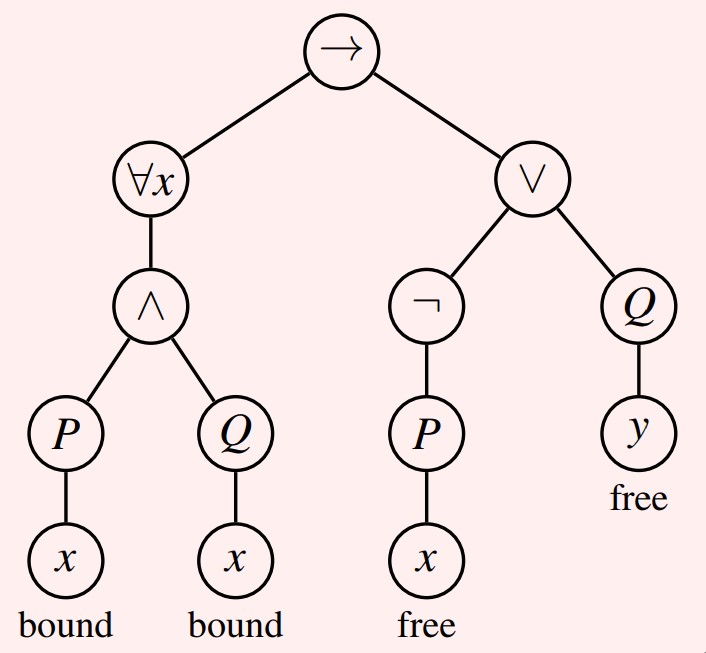
\includegraphics[width=0.5\linewidth]{fig/free_bound_var.jpg}
\end{figure}
\end{definition}
\begin{definition}[替代(substituion)]
给定变量$x$、项$t$和公式$\phi$,定义$\phi[t/x]$为将$\phi$中所有自由$x$用$t$代替
\end{definition}

\subsection{逻辑证明}
\begin{itemize}
	\item equality ($=i$)
	\[\frac{}{t=t}=i\]
	\item substitution ($=e$)
	\[\frac{t_1=t_2\qquad \phi[t_1/x]}{\phi[t_2/x]}=e\]
	\item for-eliminating ($\forall x\quad e$)
	\[\frac{\forall x\phi}{\phi[t/x]}\forall x\quad e\]
	\item for-introduction ($\forall x\quad i$)
	\[\frac{\fbox{\begin{tabular}{c}$x_0$(fresh/dummy var)\\$\vdots$\\$\phi[x_0/x]$\end{tabular}}}{\forall x\phi}\forall x\quad i\]
	\item exists-introduction ($\exists x\quad i$)
	\[\frac{\phi[t/x]}{\exists x\phi}\exists x\quad i\]
	\item exists-elimination ($\exists e$)
	\[\frac{\exists x\phi\quad \fbox{\begin{tabular}{c}$x_0$\quad $\phi[x_0/x]$\\$\vdots$\\$\chi$\end{tabular}}}{\chi}\exists e\]
\end{itemize}
\begin{example}
证明$\forall x(P(x)\to Q(x)),\forall xP(x)\vdash\forall xQ(x)$
\end{example}
\begin{analysis}
推理过程如下
\begin{center}
\begin{tabular}{lll}
1 & $\forall x(P(x)\to Q(x))$ & premise\\
2 & $\forall xP(x)$ & premise\\
3 & $P(x_0)\to Q(x_0)$ & $\forall x\quad e\quad 1$\\
4 & $P(x_0)$ & $\forall x\quad e\quad 2$\\
5 & $Q(x_0)$ & $\to e\quad 3,4$\\
6 & $\forall xQ(x)$ & $\forall x\quad i\quad 3-5$
\end{tabular}
\end{center}
\end{analysis}
\begin{theorem}[等价性(equivalence)]
令$\phi$和$\psi$都为谓词逻辑的公式,有以下等价性
\[\lnot\forall x\phi\dashv\vdash\exists x\lnot\phi,\qquad\lnot\exists x\phi\dashv\vdash\forall x\lnot\phi\]
\end{theorem}

\subsection{语义}
\begin{definition}[模型(model)]
令$\mathcal{F}$为函数符号的集合,$\mathcal{P}$为谓词符号的集合。
关于$(\mathcal{F},\mathcal{P})$的模型$\mathcal{M}$包含以下数据:
\begin{itemize}
	\item 非空集合$A$
	\item 对于每一空函数符号$f\in\mathcal{F},f^{\mathcal{M}}\in A$
	\item 对于每一$f\in\mathcal{F}$且元$n>0$,具体函数$f^{\mathcal{M}}:A^n\to A$
	\item 对于每一$P\in\mathcal{P}$且元$n>0$,子集$P^\mathcal{M}\subset A^n$
\end{itemize}
\end{definition}

\subsection{不可判定性}
